% Made up for the tikra benchmark.
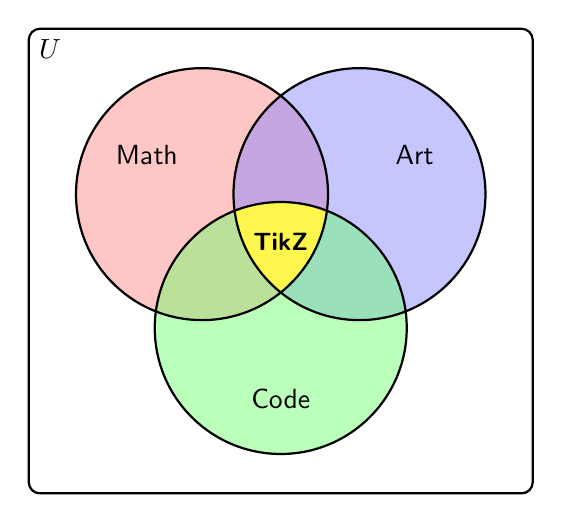
\begin{tikzpicture}[font=\sffamily, thick]
  \def\ra{(0,0) circle (1.6)}
  \def\rb{(2,0) circle (1.6)}
  \def\rc{(1,-1.7) circle (1.6)}
  \fill[red!50, opacity=0.45] \ra;
  \fill[blue!50, opacity=0.45] \rb;
  \fill[green!60, opacity=0.45] \rc;
  \begin{scope}
    \clip \ra; \clip \rb; \fill[yellow!70] \rc;
  \end{scope}
  \draw \ra \rb \rc;
  \node at (-0.7,0.5) {Math};
  \node at (2.7,0.5) {Art};
  \node at (1,-2.6) {Code};
  \node[font=\sffamily\bfseries\small] at (1,-0.6) {TikZ};
  \draw[rounded corners] (-2.2,-3.8) rectangle (4.2,2.1);
  \node[anchor=north west] at (-2.2,2.1) {$U$};
\end{tikzpicture}
